\chapter{Introduction to Object-Oriented Programming (OOP) in Python}

\section{Introduction: Real-Life Hook}

Think about situations students face in daily life:

\begin{itemize}
    \item Managing student profiles with name, age, and grades  
    \item Storing information about books in a library  
    \item Tracking cars in a school parking lot  
\end{itemize}

Instead of handling each entity separately, \textbf{OOP lets us create “blueprints” called classes} and make multiple objects from them. This keeps code \textbf{organized and reusable}.

\section{Concept: What is OOP?}

\begin{definition}{Object-Oriented Programming (OOP)}
OOP is a programming paradigm that organizes code into \textbf{objects}, each representing real-world entities with \textbf{attributes (data)} and \textbf{methods (functions)}.
\end{definition}

- \textbf{Class:} Blueprint for objects  
- \textbf{Object:} Instance of a class  
- \textbf{Attribute:} Property of an object  
- \textbf{Method:} Function inside a class that performs actions  

\section{Creating a Class and Object}

\begin{verbatim}
# Class definition
class Student:
    def __init__(self, name, age, grade):
        self.name = name
        self.age = age
        self.grade = grade

    def introduce(self):
        print(f"My name is {self.name}, I am {self.age} years old, and my grade is {self.grade}")

# Creating objects
student1 = Student("Amina", 15, 9)
student2 = Student("Rafi", 16, 10)

# Calling methods
student1.introduce()
student2.introduce()
\end{verbatim}

- \texttt{\_\_init\_\_} is the \textbf{constructor} — runs when object is created  
- \texttt{self} refers to the current object  

\section{Mini-Project: Library Book Manager}

Concept:

\begin{itemize}
    \item Each book is an object with \textbf{title, author, and status (available/borrowed)}  
    \item Class methods to \textbf{borrow, return, or display info}  
\end{itemize}

Example:

\begin{verbatim}
class Book:
    def __init__(self, title, author):
        self.title = title
        self.author = author
        self.available = True

    def borrow(self):
        if self.available:
            self.available = False
            print(f"You borrowed {self.title}")
        else:
            print(f"{self.title} is already borrowed")

    def return_book(self):
        self.available = True
        print(f"You returned {self.title}")

    def info(self):
        status = "Available" if self.available else "Borrowed"
        print(f"{self.title} by {self.author} - {status}")

# Example usage
book1 = Book("Python Basics", "Mahmudun Hasan")
book2 = Book("Data Science 101", "Sara Khan")

book1.info()
book1.borrow()
book1.info()
book1.return_book()
book1.info()
\end{verbatim}

\section{Inheritance: Reusing Code}

\begin{verbatim}
# Base class
class Vehicle:
    def __init__(self, brand):
        self.brand = brand

    def start(self):
        print(f"{self.brand} vehicle is starting")

# Derived class
class Car(Vehicle):
    def honk(self):
        print(f"{self.brand} car says beep beep!")

my_car = Car("Toyota")
my_car.start()
my_car.honk()
\end{verbatim}

- Child class \textbf{inherits attributes and methods} from parent class  
- Helps \textbf{reuse code} and \textbf{organize programs}  

\section{Step-by-Step Diagram: OOP Workflow}

\begin{center}
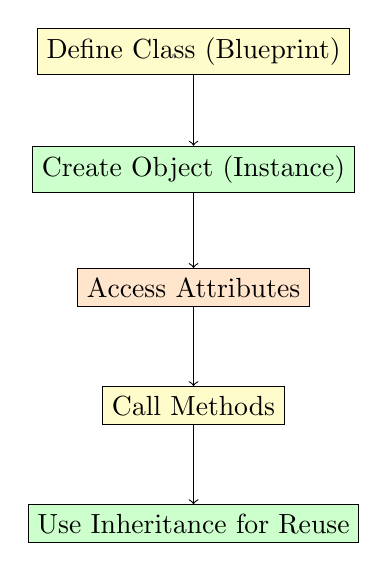
\begin{tikzpicture}[node distance=1.5cm]
\node (class) [draw, rectangle, fill=yellow!20] {Define Class (Blueprint)};
\node (object) [draw, rectangle, fill=green!20, below of=class] {Create Object (Instance)};
\node (attribute) [draw, rectangle, fill=orange!20, below of=object] {Access Attributes};
\node (method) [draw, rectangle, fill=yellow!20, below of=attribute] {Call Methods};
\node (inheritance) [draw, rectangle, fill=green!20, below of=method] {Use Inheritance for Reuse};
\draw[->] (class) -- (object);
\draw[->] (object) -- (attribute);
\draw[->] (attribute) -- (method);
\draw[->] (method) -- (inheritance);
\end{tikzpicture}
\end{center}

\section{Key Concepts}

\begin{itemize}
    \item OOP organizes code into \textbf{classes and objects}  
    \item Attributes hold \textbf{data}, methods hold \textbf{functions}  
    \item \texttt{\_\_init\_\_} constructor initializes object data  
    \item \textbf{Inheritance} allows code reuse and extension  
    \item OOP is useful for \textbf{large projects and real-life modeling}
\end{itemize}

\section{End-of-Chapter Exercises}

\begin{exercise}{Very Short Questions}
\begin{enumerate}
    \item What is a class?  
    \item What is an object?  
    \item What does the \texttt{\_\_init\_\_} method do?  
\end{enumerate}
\end{exercise}

\begin{exercise}{Short Answer Questions}
\begin{enumerate}
    \item Write a class \texttt{Student} with attributes name, age, grade and a method to display info.  
    \item Explain inheritance with an example.  
    \item How do you call a method of an object?  
\end{enumerate}
\end{exercise}

\begin{exercise}{Activity-Based Questions}
\begin{enumerate}
    \item Create a class \texttt{Animal} with methods \texttt{eat} and \texttt{sleep}. Then create a subclass \texttt{Dog} with method \texttt{bark}.  
    \item Build a class \texttt{BankAccount} with methods \texttt{deposit}, \texttt{withdraw}, and \texttt{check\_balance}.  
    \item Create a mini-library system where students can borrow and return books using classes and objects.  
\end{enumerate}
\end{exercise}

\section{Teacher Notes}

\marginnote{
\textbf{Learning Objectives:}  
\begin{itemize}
    \item Students understand classes, objects, attributes, and methods  
    \item Students can implement OOP concepts in Python  
    \item Students understand inheritance for code reuse  
\end{itemize}

\textbf{Teaching Tips:}  
\begin{itemize}
    \item Start with real-life examples like students, books, or vehicles  
    \item Emphasize the difference between class and object  
    \item Demonstrate inheritance with simple parent-child examples  
\end{itemize}

\textbf{Assessment:}  
\begin{itemize}
    \item Observe correct class and object creation  
    \item Check understanding of attributes, methods, and inheritance  
\end{itemize}
}